% Olympus v2 — Astraea inference service (astraea_service.py)
% astraea_service.tex — a per-flow sidecar inference process: __main__ is
% handed a live TCP socket fd + the exported policy via ASTRAEA_* env vars,
% builds a TF1 actor once, then a 30 ms worker thread reads flow state with
% getsockopt(tcp_deepcc_info), runs it through the recurrent policy, maps the
% action to a cwnd, and writes it back with setsockopt(cwnd). A second thread
% reads a control pipe to toggle actuation on/off at runtime.
% Compile standalone:  pdflatex astraea_service.tex
\documentclass[tikz,border=5pt]{standalone}
\usepackage{tikz}
\usepackage{amssymb}
\usepackage{helvet}
\renewcommand{\familydefault}{\sfdefault}
\usetikzlibrary{arrows.meta,positioning,fit,backgrounds}

\begin{document}
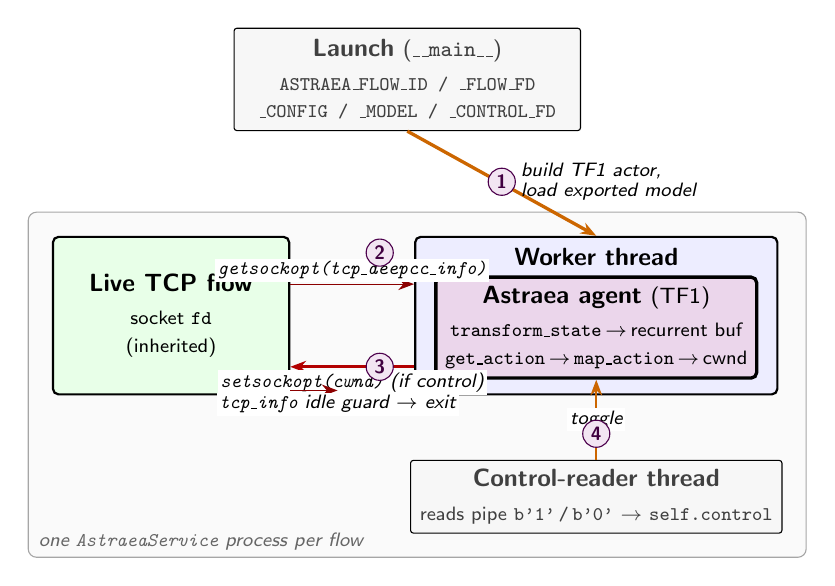
\begin{tikzpicture}[
  font=\small,
  >={Stealth[length=2mm]},
  proc/.style={draw,rounded corners=2pt,thick,minimum height=8mm,
               minimum width=24mm,align=center,fill=blue!7},
  net/.style={draw,rounded corners=2pt,thick,minimum height=8mm,
              minimum width=30mm,align=center,fill=green!9},
  agent/.style={proc,fill=violet!16,very thick},
  bridge/.style={draw,solid,thin,rounded corners=1pt,
                 minimum height=8mm,minimum width=24mm,align=center,
                 fill=black!3,text=black!75},
  subbox/.style={draw,rounded corners=1.5pt,thin,draw=violet!60,fill=white,
                 font=\scriptsize,inner sep=2pt,
                 minimum width=15mm,minimum height=4.5mm},
  band/.style={draw,rounded corners=3pt,thin,draw=black!35,fill=black!2},
  stepnum/.style={circle,draw=violet!60!black,fill=violet!10,inner sep=0.45mm,
                  font=\scriptsize\bfseries,text=violet!50!black},
  data/.style={->,very thick,draw=red!70!black},
  tap/.style={->,thin,draw=red!55!black},
  cfg/.style={->,thick,draw=orange!80!black},
  lbl/.style={font=\scriptsize\itshape,fill=white,inner sep=1pt},
]

% ---- top: process launch, handed the flow + model through the environment ----
\node[bridge,minimum width=44mm,minimum height=13mm] (main) at (24mm,26mm)
     {\textbf{Launch} \footnotesize(\texttt{\_\_main\_\_})\\[1pt]
      \scriptsize \texttt{ASTRAEA\_FLOW\_ID / \_FLOW\_FD}\\[-1pt]
      \scriptsize \texttt{\_CONFIG / \_MODEL / \_CONTROL\_FD}};

% ---- left: the live TCP flow whose fd was inherited ----
\node[net,minimum width=30mm,minimum height=20mm] (flow) at (-6mm,-4mm)
     {\textbf{Live TCP flow}\\[1pt]
      \scriptsize socket \texttt{fd}\\[-1pt]
      \scriptsize (inherited)};

% ---- centre: the worker's 30 ms control loop ----
\node[proc,minimum width=46mm,minimum height=20mm] (worker) at (48mm,-4mm) {};
\node[align=center,anchor=north,inner sep=0pt] at ([yshift=-1.5mm]worker.north)
     {\textbf{Worker thread}\\[-1pt]
      \scriptsize \texttt{\_run\_flow} — every 30\,ms};

% the policy actor lives inside the loop
\node[agent,minimum width=40mm,minimum height=8.5mm,anchor=south]
     at ([yshift=2mm]worker.south) (agent)
     {\textbf{Astraea agent} \footnotesize(TF1)\\[1pt]
      \scriptsize \texttt{transform\_state}\,$\to$\,recurrent buf\\[-1pt]
      \scriptsize \texttt{get\_action}\,$\to$\,\texttt{map\_action}\,$\to$\,cwnd};

% ---- bottom: control-reader thread fed by the orchestrator's pipe ----
\node[bridge,minimum width=46mm,minimum height=9mm] (ctrl) at (48mm,-27mm)
     {\textbf{Control-reader thread}\\[1pt]
      \scriptsize reads pipe \texttt{b'1'\,/\,b'0'} $\to$ \texttt{self.control}};

% backdrop card: everything after launch is one AstraeaService process
\begin{scope}[on background layer]
  \node[band,fit=(flow)(worker)(agent)(ctrl),inner sep=3mm] (proc) {};
\end{scope}
\node[font=\scriptsize\itshape,text=black!60,anchor=south west,fill=black!2,
      inner sep=1pt] at ([xshift=1mm,yshift=0.6mm]proc.south west)
     {one \texttt{AstraeaService} process per flow};

% (1) launch builds the service and loads the exported model once
\draw[cfg,very thick] (main.south) -- (worker.north);
\node[stepnum] at (36mm,13mm) {1};
\node[align=left,anchor=west,font=\scriptsize\itshape,inner sep=1pt]
     at (38mm,13mm) {build TF1 actor,\\[-1pt]load exported model};

% (2) read flow state each tick
\draw[tap] ([yshift=4mm]flow.east) -- node[lbl,above=0.2mm]{\texttt{getsockopt(tcp\_deepcc\_info)}}
      ([yshift=4mm]worker.west);
\node[stepnum] at (20.5mm,4mm) {2};

% (3) act on the flow — only while control is enabled
\draw[data] ([yshift=-6.5mm]worker.west)
      -- node[lbl,below=0.2mm]{\texttt{setsockopt(cwnd)} \scriptsize(if control)}
      ([yshift=-6.5mm]flow.east);
\node[stepnum] at (20.5mm,-10.5mm) {3};

% (4) idle guard: poll tcp_info, exit the process when the flow goes quiet
\draw[tap] ([yshift=-9.5mm]flow.east) -- ([yshift=-9.5mm,xshift=6mm]flow.east)
      node[lbl,below=0.2mm,anchor=north]{\texttt{tcp\_info} idle guard $\to$ exit};

% control pipe toggles actuation
\draw[cfg] (ctrl.north) -- node[lbl]{toggle} (agent.south);
\node[stepnum] at (48mm,-19mm) {4};

\end{tikzpicture}
\end{document}
